\begin{center}
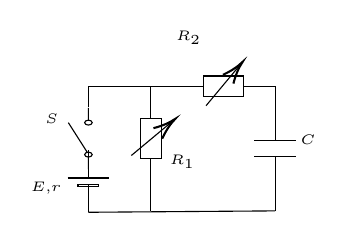
\begin{tikzpicture}[x=0.75pt,y=0.75pt,yscale=-1,xscale=1]
%uncomment if require: \path (0,300); %set diagram left start at 0, and has height of 300

%Shape: Battery [id:dp9725213714143768] 
\draw   (120,180.67) -- (120,167.17) (110,164.17) -- (130,164.17) (120,164.17) -- (120,150.67) (115,168.37) -- (115,167.17) -- (125,167.17) -- (125,168.37) -- (115,168.37) -- cycle ;
%Shape: Simple Switch [id:dp9513460496272634] 
\draw   (120,160) -- (120,154.07) (120,136.29) -- (120,130.37) (119.39,151.7) -- (110.32,137.48) (120,138.66) .. controls (119,138.66) and (118.18,138.13) .. (118.18,137.48) .. controls (118.18,136.82) and (119,136.29) .. (120,136.29) .. controls (121,136.29) and (121.82,136.82) .. (121.82,137.48) .. controls (121.82,138.13) and (121,138.66) .. (120,138.66) -- cycle (120,154.07) .. controls (119,154.07) and (118.18,153.54) .. (118.18,152.89) .. controls (118.18,152.23) and (119,151.7) .. (120,151.7) .. controls (121,151.7) and (121.82,152.23) .. (121.82,152.89) .. controls (121.82,153.54) and (121,154.07) .. (120,154.07) -- cycle ;
%Straight Lines [id:da13406352029154833] 
\draw    (120,130) -- (120,120) ;
%Shape: Resistor [id:dp7782080231234687] 
\draw   (145,154.6) -- (145,135.4) -- (155,135.4) -- (155,154.6) -- (145,154.6) -- cycle (150,160) -- (150,154.6) (150,135.4) -- (150,130) ;
%Straight Lines [id:da13059673417265527] 
\draw    (140.67,153.33) -- (160.3,136.96) ;
\draw [shift={(161.84,135.67)}, rotate = 140.17] [color={rgb, 255:red, 0; green, 0; blue, 0 }  ][line width=0.75]    (10.93,-3.29) .. controls (6.95,-1.4) and (3.31,-0.3) .. (0,0) .. controls (3.31,0.3) and (6.95,1.4) .. (10.93,3.29)   ;

%Straight Lines [id:da15333654490325355] 
\draw    (120,120) -- (170,120) ;
%Straight Lines [id:da8531691012035736] 
\draw    (150,130) -- (150,120) ;
%Straight Lines [id:da4440724028211367] 
\draw    (150,180) -- (150,160) ;
%Shape: Resistor [id:dp2809007889817905] 
\draw   (175.4,125) -- (194.6,125) -- (194.6,115) -- (175.4,115) -- (175.4,125) -- cycle (170,120) -- (175.4,120) (194.6,120) -- (200,120) ;
%Straight Lines [id:da8392657712741902] 
\draw    (176.67,129.33) -- (193.04,109.7) ;
\draw [shift={(194.33,108.16)}, rotate = 129.83] [color={rgb, 255:red, 0; green, 0; blue, 0 }  ][line width=0.75]    (10.93,-3.29) .. controls (6.95,-1.4) and (3.31,-0.3) .. (0,0) .. controls (3.31,0.3) and (6.95,1.4) .. (10.93,3.29)   ;

%Straight Lines [id:da5062655598048114] 
\draw    (200,120) -- (210,120) -- (210,140) ;
%Shape: Contact [id:dp3034505709269577] 
\draw   (210,140) -- (210,146) (210,160) -- (210,154) (220,146) -- (200,146) (220,154) -- (200,154) ;
%Straight Lines [id:da6904084679904827] 
\draw    (210,180) -- (210,160) ;
%Straight Lines [id:da5835108292810021] 
\draw    (120,180.67) -- (210,180) ;

% Text Node
\draw (91,165) node [anchor=north west][inner sep=0.75pt]  [font=\tiny] [align=left] {$\displaystyle E$,$\displaystyle r$};
% Text Node
\draw (98,132) node [anchor=north west][inner sep=0.75pt]  [font=\tiny] [align=left] {$\displaystyle S$};
% Text Node
\draw (158,152) node [anchor=north west][inner sep=0.75pt]  [font=\tiny] [align=left] {$\displaystyle R_{1}$};
% Text Node
\draw (161,92) node [anchor=north west][inner sep=0.75pt]  [font=\tiny] [align=left] {$\displaystyle R_{2}$};
% Text Node
\draw (221,142) node [anchor=north west][inner sep=0.75pt]  [font=\tiny] [align=left] {$\displaystyle C$};


\end{tikzpicture}

\end{center}